 
\documentclass[DIN, pagenumber=false, fontsize=11pt, parskip=half]{scrartcl}

\usepackage{amsmath}
\usepackage{amsfonts}
\usepackage{amssymb}
\usepackage{enumitem}
\usepackage[utf8]{inputenc} % this is needed for umlauts
\usepackage[ngerman]{babel} % this is needed for umlauts
\usepackage[T1]{fontenc} 
\usepackage{commath}
\usepackage{xcolor}
\usepackage{booktabs}
\usepackage{float}
\usepackage{tikz-timing}
\usepackage{tikz}
\usepackage{multirow}
\usepackage{colortbl}
\usepackage{xstring}
\usepackage{circuitikz}
\usepackage{listings} % needed for the inclusion of source code
\usepackage[final]{pdfpages}
\usepackage{subcaption}

\usetikzlibrary{calc,shapes.multipart,chains,arrows}

\newcommand{\Prb}[1]{P(\text{#1})}
\newcommand{\CPr}[2]{P(\text{#1}|\text{#2})}
\DeclareMathOperator*{\argmax}{arg\,max}
\DeclareMathOperator*{\argmin}{arg\,min}

\title{Pattern Recognition}
\author{Tim Luchterhand, Paul Nykiel, Jonas Strauch (Group P)}

\begin{document}
    \maketitle
    \section{Decision Surfaces via Gaussian Density Functions [Pen and Paper]}
    \begin{table}[H]
        \centering
        \begin{tabular}{cccccc}
            \toprule
            $\mu_1$ & $\Sigma_1$ & $\mu_2$ & $\Sigma_2$ & Decision Surface & Slice \\
            \midrule
            $\begin{pmatrix} 0 \\ 0 \end{pmatrix}$ & $\begin{pmatrix} 1 & 0 \\ 0 & 1 \end{pmatrix}$ &
                $\begin{pmatrix} 2 \\ 0 \end{pmatrix}$ & $\begin{pmatrix} 3 & 0 \\ 0 & 3 \end{pmatrix}$ &
                (b) & (e)  \\
            $\begin{pmatrix} 0 \\ 0 \end{pmatrix}$ & $\begin{pmatrix} 1 & 0 \\ 0 & 1 \end{pmatrix}$ &
                $\begin{pmatrix} 2 \\ 0 \end{pmatrix}$ & $\begin{pmatrix} 1 & 0 \\ 0 & 3 \end{pmatrix}$ &
                (c) & (f) \\
            $\begin{pmatrix} 0 \\ 0 \end{pmatrix}$ & $\begin{pmatrix} 2 & 0 \\ 0 & 3 \end{pmatrix}$ &
                $\begin{pmatrix} 2 \\ 0 \end{pmatrix}$ & $\begin{pmatrix} 6 & 0 \\ 0 & 1 \end{pmatrix}$ &
                (a) & (d) \\
            \bottomrule
        \end{tabular}
        \caption{Parameters for the Gaussian functions which define the decision surfaces.}
    \end{table}
    
    \paragraph{First Row}
    Both gaussian distributions have covariance matrices that are multiples of the identity matrix. 
    The first gaussian is centered around $(0,0)$, with a variance of $1$, the second gaussian is centred around $(2,0)$ with a variance of $3$.
    Therefore the difference between $\sigma_x^2$ of both gaussians is larger than the in the second row which means that the corresponding slice
    is shown in subfigure (e) as opposed to (f). Subfigure (d) is not possible either because it belongs to the third row as explained shortly.
    Looking at these graphs it can be seen that all points right of approx. $x_1 = 2$ are classified as class two.
    Additionally all points on the far left (approx. $x_1 < 5$) are classified as class two as well due to the higher variance of the gaussian of class two.
    Further more since both gaussians have multiples of the identity as covariance matrices, the decision surface takes the shape of a circle which can be seen
    subfigure (b).

    \paragraph{Second row}
    The gaussian distributions that are listed in the second row both have a variance of $1$ along the $x_1$ axis. This can be seen in slice (f) where both
    gaussians have the same width along the $x_1$ axis.
    Additionally, this yields one decision boundary along the $x_1$ axis (which is still dependent one the $x_2$ value).
    These properties can be seen in subfigure (f) (the decision boundary is at approx. $2$), and subfigure (c).

    \paragraph{Third row}
    The variance of the first gaussian distribution along the $x_2$ axis is larger than the variance of the second distribution along the $x_2$ axis.
    These properties can only be seen in subfigure (d). This graph shows that there is an area parallel to the $x_1$ axis completely belonging to class one.
    This can only be seen in subfigure (a).

    \section{Euclidean Distance, Standardization, Mahalanobis Distance}
    \subsection{}
    \begin{enumerate}[label=\alph*)]
        \item In the Figure the closest point to $(1,1200)$ is $(1.5,1000)$
        \item The closest point is not the point which seems to be the closest in the figure. This is due to the fact that the two axis are not scaled the same. 
            As a result the distance in $y$-direction (monthly income), is of much higher importance than the distance in $x$-direction (years of education).
    \end{enumerate}

    \subsection{}
    \begin{enumerate}[label=\alph*)]
        \item For a random variable $x$ let $U$ denote the unit of this variable. The unit of the variance $\mu_x$ of this random variable is thus $U$ as well.
            The unit of the variance of a random variable is given by:
            \begin{eqnarray*}
                [\sigma_x^2] &=& \left[\frac{1}{n-1} \cdot \sum_{i=1}^n {(x_i - \mu_x)}^2\right] \\
                &=& \left[\frac{1}{n-1}\right] \cdot \sum_{i=1}^n \left[{(x_i - \mu_x)}^2\right] \\
                &=& 1 \cdot {([x_i - \mu_x])}^2 \\
                &=& 1 \cdot U^2 \\
                &=& U^2
            \end{eqnarray*}
            Thus the unit of the standard deviation $\sigma_x = \sqrt{\sigma_x^2}$ is the same as the unit of the random variable $\sqrt{U^2} = U$.
            As a result $\tilde{x}$ is unitless: $[\tilde{x}] = [\frac{x - \mu_x}{\sigma_x}] = 1$.
        \item By normalizing the random variables by their respective standard deviation the standard deviation and thus the variance of the data is $1$.
            This yields random variables with equal scale, and as a result the distance between the points is not biased towards one variable.
        \item The $x_i$ and $x_j$ that are given in the exercise are refered to as $x$ and $y$ in this proof to avoid confusion with the subscripts used for element indexing.
            \begin{eqnarray*}
                d_E(\tilde{x}, \tilde{y}) &=& \norm{\tilde{x} - \tilde{y}}_2 \\
                    &=& \sqrt{{(\tilde{x}_1 - \tilde{y}_1)}^2 + {(\tilde{x}_2 - \tilde{y}_2)}^2} \\
                    &=& \sqrt{{\left(\frac{x_1 - \mu_1}{\sigma_1} - \frac{y_1 - \mu_1}{\sigma_1}\right)}^2 + {\left(\frac{x_2 - \mu_2}{\sigma_2} - \frac{y_2 - \mu_2}{\sigma_2}\right)}^2} \\
                    &=& \sqrt{{\left(\frac{x_1 - \mu_1 - (y_1 - \mu_1)}{\sigma_1}\right)}^2 + {\left(\frac{x_2 - \mu_2 - (y_2 - \mu_2)}{\sigma_2}\right)}^2} \\
                    &=& \sqrt{{\left(\frac{x_1 - y_1}{\sigma_1}\right)}^2 + {\left(\frac{x_2 - y_2}{\sigma_2}\right)}^2} \\
                    &=& \sqrt{\frac{{(x_1 - y_1)}^2}{\sigma_1^2} + \frac{{(x_2 - y_2)}^2}{\sigma_2^2}} \\
                    &=& \sqrt{
                        \begin{pmatrix}x_1 - y_1 & x_2 - y_2 \end{pmatrix} 
                            \begin{pmatrix} \frac{1}{\sigma_1^2} & 0 \\ 0 & \frac{1}{\sigma_2^2} \end{pmatrix} 
                            \begin{pmatrix}x_1 - y_1 \\ x_2 - y_2 \end{pmatrix}}\\
                    &=& \sqrt{{(x-y)}^\text{T}
                            {\begin{pmatrix} \sigma_1^2 & 0 \\ 0 & \sigma_2^2 \end{pmatrix}}^{-1}
                            (x-y)} \\
                    &=& \sqrt{{(x-y)}^\text{T}
                            S^{-1}
                            (x-y)} \\
                    &=& d_S(x,y)
            \end{eqnarray*}
    \end{enumerate}

    \subsection{}
    \begin{figure}[H]
        \centering
        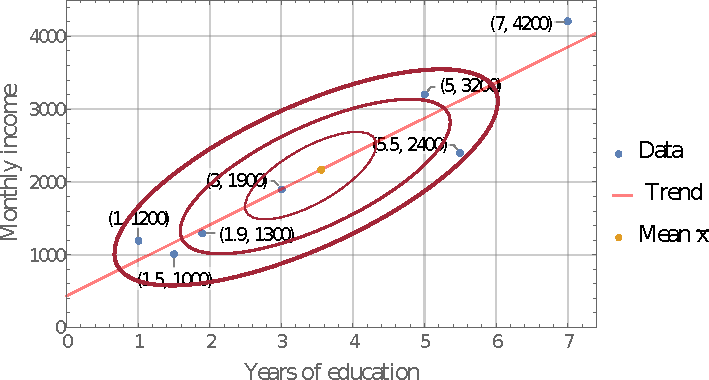
\includegraphics[width=\textwidth]{A3_1.pdf}
        \caption{Plot of the data points and the isocurve (in red) around the mean}
    \end{figure}

    \begin{figure}[H]
        \centering
        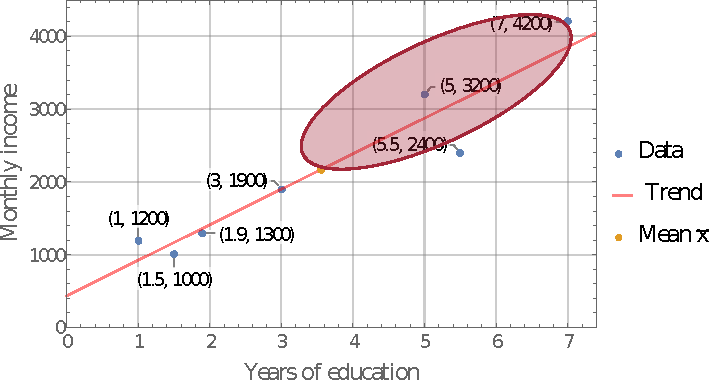
\includegraphics[width=\textwidth]{A3_2.pdf}
        \caption{Plot of the data points and the isocurve (in red) around (5,3200)}
    \end{figure}
    By moving the isocurve around $(5,3200)$ it can be seen, that $(7,4200)$ is on the isocurve and $(5.5,2400)$ is outside of the isocurve. Thus the distance of $(5,3200)$ to $(7,4200)$ is smaller than the distance to $(5.5,2400)$.
    

    \subsection{}
    \lstinputlisting[language=Python]{distance.py}
\end{document}
